%\documentclass[11pt,twocolumn,twoside]{article}
\documentclass[11pt,twoside]{article}

\usepackage{anysize}
\usepackage{fancyvrb}
%\usepackage{fancyhdr}
\usepackage{color}
%\usepackage{multicol}
\usepackage{graphicx}

\definecolor{code}{gray}{0.75}
\newcommand{\printcommand}[1]{\colorbox{code}{\scriptsize{\BUseVerbatim{#1}}}}

%\newcommand{\url}[1]{{\tiny{#1}}}

\marginsize{3cm}{2cm}{2cm}{2cm}
\setlength\oddsidemargin{0cm}
\setlength\evensidemargin{0cm}

\setlength\columnseprule{.4pt}

\begin{document}

\title{Genes underlying inheritance linked disorders (GUILD) framework - Software Handbook}
%\title{GUILD framework: Network based prioritization of disease candidate genes}
\author{Emre G\"{u}ney\footnote{Structural Bioinformatics Laboratory, Pompeu Fabra University, \today}}
\date{}
\maketitle

%\begin{center}
%\section*{Introduction}
%\end{center}

GUILD (Genes Underlying Inheritance Linked Disorders) is a framework built for 
the prioritization of disease candidate genes using a priori gene-disease 
associations and protein interactions. 
GUILD consists of implementations of 8 algorithms: NetScore, NetZcore, NetShort,
NetCombo, fFlow, NetRank, NetWalk and NetProp. NetScore, NetZcore, NetShort, 
fFlow and NetRank are implemented in \textit{C++} while NetWalk and NetProp 
are implemented in \textit{R} and NetCombo is a \textit{Python} script combining
the results of NetScore, NetZcore and NetShort.
In this manual, we describe how to use these programs included in GUILD framework.

\tableofcontents

%\vspace{1cm}

%\begin{multicols}{2}


\section{Requirements}

\begin{itemize}
\item GCC (GNU project C/C++ compiler) (version 4.3 or higher)
\item make (GNU project utility to maintain groups of programs)
%\item Boost Graph Library (BGL) (version 1.41 or higher)
\item R (version 2.12.1 or higher) \textit{(only required for running NetWalk and NetProp)}
\end{itemize}

Unix-like operating systems typically ship with these programs. If not these
programs are freely available online. Note that, Windows users can have the 
fundamental environment for the installation (\textit{GCC} and \textit{make}) 
through {\it{MinGW}} (http://www.mingw.org) or {\it{Cygwin}} 
(http://www.cygwin.com).
%Boost Graph Library (BGL) is a free header based C++ library (part of Boost 
%C++ libraries, http://www.boost.org) and no separate installation is required 
%once you download the library files. However, you will need the directory 
%where Boost libraries are located for the installation step.
\textit{R} is a free software environment for statistical computing and 
graphics and available at http://www.r-project.org/.


\section{Installation}

Download and unpack the source package \textit{guild.tar.gz} located at 
http://sbi.imim.es/web/GUILD.php e.g. as follows

\begin{SaveVerbatim}{bash}
\$> tar xvzf guild.tar.gz
\end{SaveVerbatim}
\printcommand{bash}
%\$> wget http://sbi.imim.es/web/guild.tar.gz

\vspace{5 mm}
Then, go to the extracted directory%, issue the following commands to make the 
%compiler aware of the directory where Boost libraries are located. 
\begin{SaveVerbatim}{bash}
\$> cd guild
\end{SaveVerbatim}
\printcommand{bash}
%\$> export BGL_PATH=path_to_boost_library

\vspace{5 mm}
Next, go to the src folder and issue \textit{make} command as below. Beware 
that \textit{make} command in MinGW can have a different name (e.g. 
\textit{mingw32-make.exe})
\begin{SaveVerbatim}{bash}
\$> cd src 
\$> make
\end{SaveVerbatim}
\printcommand{bash}

\vspace{5 mm}
An executable named \textit{guild} should be created under the ``guild'' folder.
Try running it as follows

\begin{SaveVerbatim}{bash}
\$> cd ..
\$> ./guild
\end{SaveVerbatim}
\printcommand{bash}

\vspace{5 mm}
If you get the following output when you run it, the installation is successfully 
completed. 

\begin{SaveVerbatim}{bash}
./guild [ Copyleft (GPLv3) - 2011 - Emre Guney (Universitat Pompeu Fabra) ]

 Arguments: 
     -s <prioritization_method>{NetScore:s|NetZcore:z|NetShort:d|fFlow:f|NetRank:r}
     -n <node_file>
     -e <edge_file>
     -o <output_file>
     -i <number_of_iterations>
     -r <number_of_repetitions>
     -t <seed_score_threshold>
     -x <number_of_sampled_graphs>
     -d <sampled_graph_prefix>
     -h
\end{SaveVerbatim}
\printcommand{bash}

\vspace{5 mm}
Otherwise make sure that you have recent versions of \textit{GCC} and 
\textit{make} installed, % and \textit{BGL} installed, 
check the steps above and retry compiling.


\section{Usage}

For algorithms implemented in C++, a typical GUILD call consist of several 
mandatory arguments (such as name of the input/output files and type of the 
prioritization method) followed by prioritization method specific arguments. 
Mandatory arguments common to all prioritization methods are explained below, 
method specific arguments are described in the later sections for each method 
separately. Possible arguments for a GUILD executable call is as follows:

\begin{SaveVerbatim}{bash}
\$> ./guild -s <prioritization_method> -n <node_file> -e <edge_file> -o <output_file> 
	    -i <number_of_iterations> -r <number_of_repetitions> -t <seed_score_threshold> 
	    -x <number_of_sampled_graphs> -d <sampled_graph_prefix>
\end{SaveVerbatim}
\printcommand{bash}

\vspace{5 mm}
where;

\begin{description}
    \item[prioritization\_method:] The type of the prioritization algorithm, 
	available values are 
	\begin{itemize}
	    \item s: NetScore
	    \item z: NetZcore 
	    \item d: NetShort 
	    \item f: fFlow 
	    \item r: NetRank
	\end{itemize}

    \item[node\_file:] Input node scores file containing node (e.g. protein or 
	gene) identifier followed by its phenotypic relevance score (e.g. 
	association with the disease phenotype for that protein/gene) on each 
	line. The values need to be separated by whitespace(s). That is;
\begin{SaveVerbatim}{text}
<node_id> <node_score>
\end{SaveVerbatim}
\printcommand{text}

    \item[edge\_file:] Input edge scores file containing node (e.g. protein or 
	gene) identifier followed by score of the edge its phenotypic 
	relevance score (e.g. association with the disease phenotype for the 
	proteins/genes it is connecting) and node identifier (the interaction 
	partner) on each line. The values are separated by whitespace(s). Thus, 
	a line in this file looks like;
\begin{SaveVerbatim}{text}
<node_id> <edge_score> <node_id>
\end{SaveVerbatim}
\printcommand{text}

    \item[output\_file:] Output node scores file containing node (e.g. protein 
	or gene) identifier followed by its ``calculated'' phenotypic 
	relevance score (e.g. association with the disease phenotype for that 
	protein/gene) on each line. The values are separated by whitespace(s). 
	The format of a line would be;
\begin{SaveVerbatim}{text}
<node_id> <node_score>
\end{SaveVerbatim}
\printcommand{text}
%    \item[number\_of\_repetitions]: \textit{Only for NETSCORE.} The number of resets (updating the scores of the nodes to calculated scores so far) in the algorithm (see details in the description of the prioritization method). Defines the reach of the method (number of links to look further while calculating score) in accordance with the number\_of\_iteration parameter.
%    \item[number\_of\_iterations]: \textit{For NETSCORE, NETZCORE, FFLOW, NETRANK.} Number of iterations to apply the scoring step of the prioritization algorithm. 
%	% For NETSCORE defines the length of shortest paths to consider from a node to other nodes (messages of the nodes that are this many links further are considered).
%    \item[seed\_score\_threshold]: \textit{For FFLOW only.} All the nodes that have higher than this given threshold score will be considered as seeds for the method and assigned infinite scores during scoring.
%    \item[number\_of\_sampled\_graphs]: \textit{Only for NETZCORE.} Number of the sampled networks (random networks with similar characteristics --e.g. topology or degree distribution-- of original network) used for calculating expected mean and standard deviation of scores by random.
%    \item[sampled\_graph\_prefix]: \textit{Only for NETZCORE.} The full prefix of the sampled networks. An integer from 1 to n\_sampled\_graphs will be appended at the end of this text while reading sampled networks (thus it should include the directory under which random network files reside).

\end{description}

For algorithms implemented in R (NetWalk and NetProp), a typical GUILD call would look like:

\begin{SaveVerbatim}{bash}
\$> R --slave --args <node_file> <edge_file> <output_file> <use_propagation> < random_walk.r
\end{SaveVerbatim}
\printcommand{bash}

\vspace{5 mm}
where all arguments are as explained before except ``use\_propagation'', which --if provided-- converts NetWalk algorithm to NetProp.

\subsection{NetScore}
NetScore adopts a message-passing scheme such that each node sends the 
information associated with it as a message to all of its neighbours and the 
neighbours convey these messages to their neighbours. NetScore takes into 
consideration alternative shortest paths within the distance of at most 
number\_of\_iterations links at each so called repetition-cycle. At the end of 
the repetition cycle, the node scores are updated according to messages 
recieved so far and the message passing is restarted.

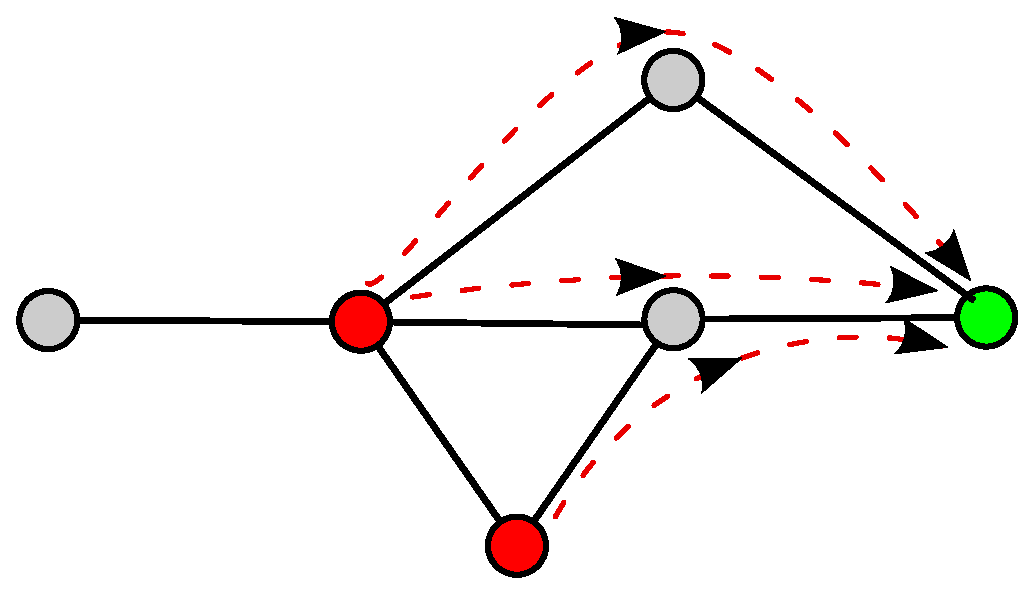
\includegraphics[scale=0.5]{netscore.eps}

\vspace{5 mm}
Method specific parameters for NetScore are;
\begin{description}
    \item[number\_of\_repetitions:] The number of resets (updating the scores 
	of the nodes to calculated scores so far) in the algorithm. Defines the 
	reach of the method (number of links to look further while calculating 
	score) in accordance with the number\_of\_iteration parameter.
    \item[number\_of\_iterations:] Number of iterations to apply the scoring 
	step of the prioritization algorithm. That is the length of shortest 
	paths to consider from a node to other nodes (messages of the nodes 
	that are this many links further are considered).
\end{description}
%These parameters may need to be optimized depending on the network and the computational resource available, however during our analysis the values that has yielded sub-optimal performance for number of iterations and repetitions were 2 and 3 respectively (achieving a coverage of $2*3=6$ links approximately).

The following is an example call to run NetScore algorithm using node file 
\textit{node\_score.txt} and edge \textit{file edge\_score.txt} with number 
of iteration and repetition parameters of \textit{2} and \textit{3} 
respectively, writing the calculated scores to a file named output.txt.

\begin{SaveVerbatim}{bash}
\$> ./guild -s s -n data/test_proteins.txt -e data/test_interactions.txt -o output.txt -r 3 -i 2
\end{SaveVerbatim}
\printcommand{bash}

\subsection{NetZcore}
NetZcore assigns a normalized score using the distribution of the scores of 
neighbouring nodes. The normalization uses a random model of networks and it 
is calculated with the Z-score formulae: z=(x-m)/s, where m is the average of 
scores of neighbouring nodes with similar distribution in the random network 
and s is the standard deviation. The distribution is obtained with hundred 
network-replicates obtained by randomly shuffling the scores among nodes with 
similar degree (i.e. 100 random networks preserving the original topology).

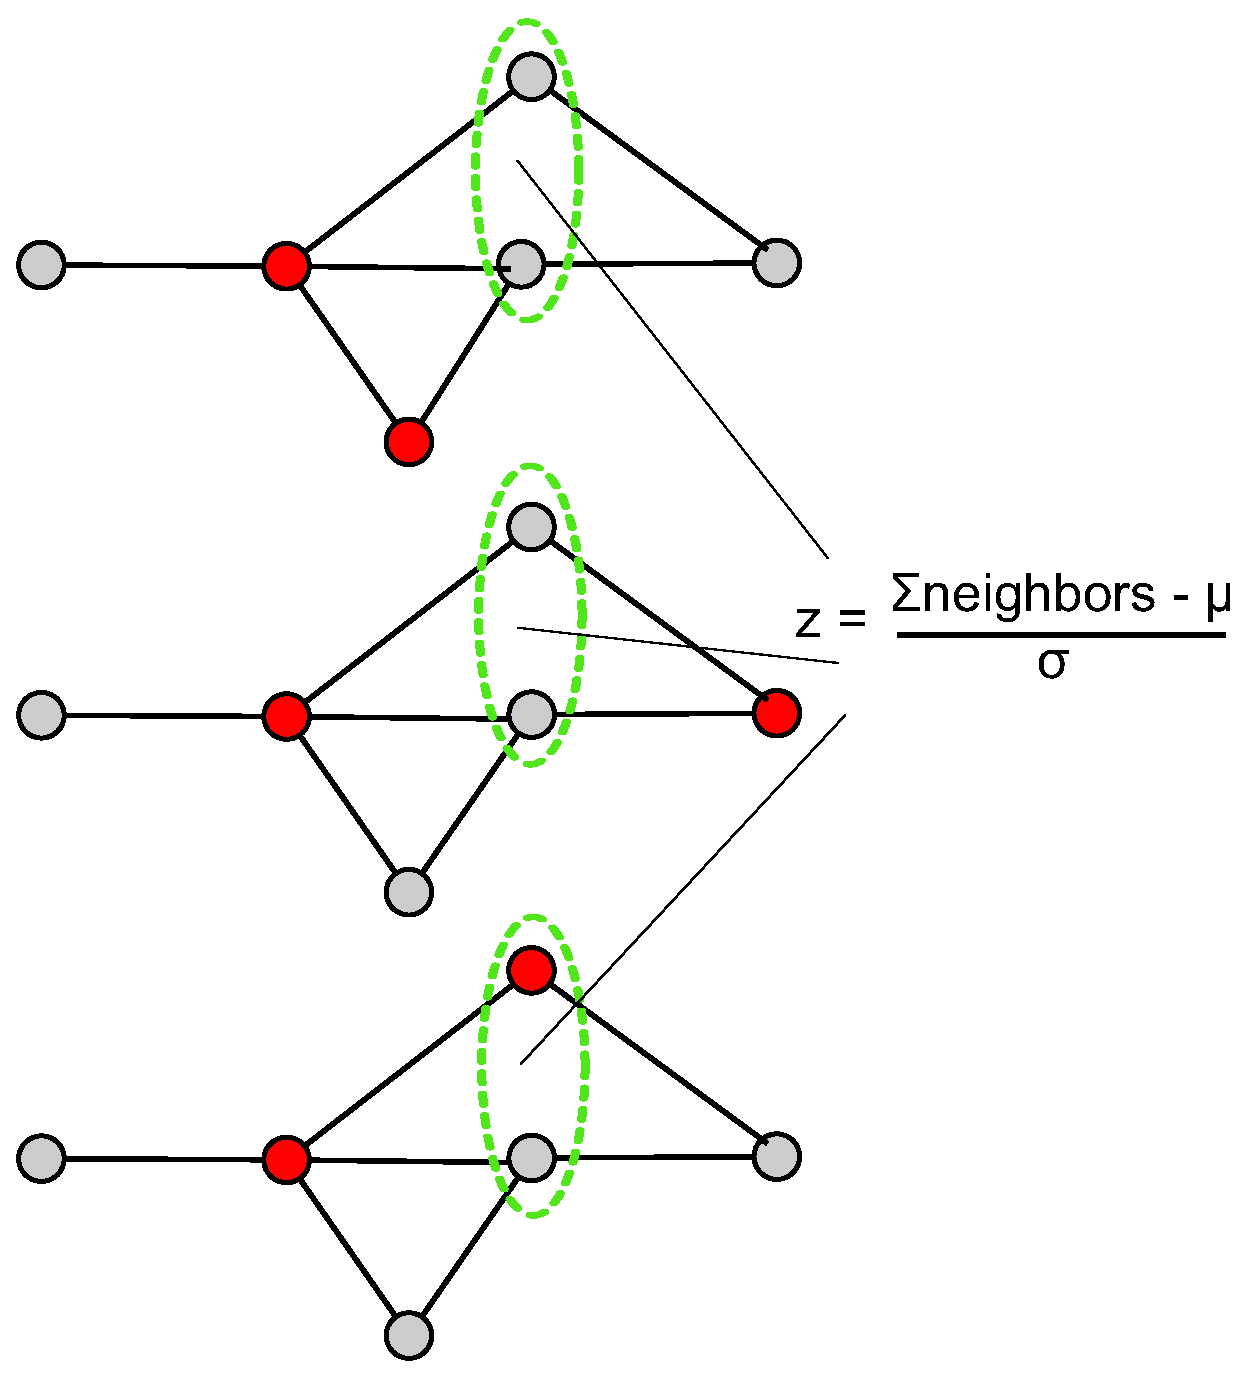
\includegraphics[scale=0.5]{netzcore.eps}

\vspace{5 mm}
Method specific parameters for NetZcore are;
\begin{description}
    \item[number\_of\_iterations:] Number of iterations to apply the scoring 
	step of the prioritization algorithm. 
    \item[number\_of\_sampled\_graphs:] Number of the sampled networks (random 
	networks with similar characteristics --e.g. topology or degree 
	distribution-- of original network) used for calculating expected mean 
	and standard deviation of scores by random.
    \item[sampled\_graph\_prefix:] The full prefix of the sampled networks. An 
	integer from 1 to n\_sampled\_graphs will be appended at the end of 
	this text while reading sampled networks (thus it should include the 
	directory under which random network files reside). Note that the 
	program itself does not create random networks and looks for already 
	existing random networks residing under the path given by this parameter.
	A python script is provided for creating such networks (see below).
\end{description}
%    You can generate random networks using graph_utilities.randomize_graph function with randomization_type "preserve_topology_and_node_degree"
%Suggested number of iterations and number of random random graphs is 5 and 100, however these values are also network specific.

An example call to run NetZcore algorithm where \textit{data} 
folder contains 100 randomly generated networks starting with the prefix 
\textit{test\_interactions.txt.} (e.g. \textit{test\_interactions.txt.1}, 
\textit{test\_interactions.txt.2}, \ldots, \textit{test\_interactions.txt.100} 
is as follows:

\begin{SaveVerbatim}{bash}
\$> ./guild -s z -n data/test_proteins.txt -e data/test_interactions.txt -o output.txt -i 5 
	    -d data/test_interactions.txt. -x 100
\end{SaveVerbatim}
\printcommand{bash}

\vspace{5 mm}
A python script named ``create\_random\_networks\_for\_netzcore.py'' is provided 
for creating random networks that are going to be used by NetZcore. It requires 
\textit{Python} (version 2.5.2 or higher) and Python \textit{NetworkX} (version 
1.1 or higher) package to be installed in your system. The following command 
would create 100 random networks with the same topology of given input network
``data/test\_interactions.txt'' with the prefix of 
``data/test\_interactions.txt.'' (appends a dot at the end of the provided egde 
scores file name).

\begin{SaveVerbatim}{bash}
\$> python src/create_random_networks_for_netzcore.py data/test_interactions.txt 100
\end{SaveVerbatim}
\printcommand{bash}

\subsection{NetShort}
NetShort accumulates the weighted shortest path lengths between a node and the 
rest of nodes in the network, where each edge-weight is inversely proportional 
to the average of the scores of the two nodes connected by the edge (i.e.edges 
connecting high scoring nodes are shorter). 

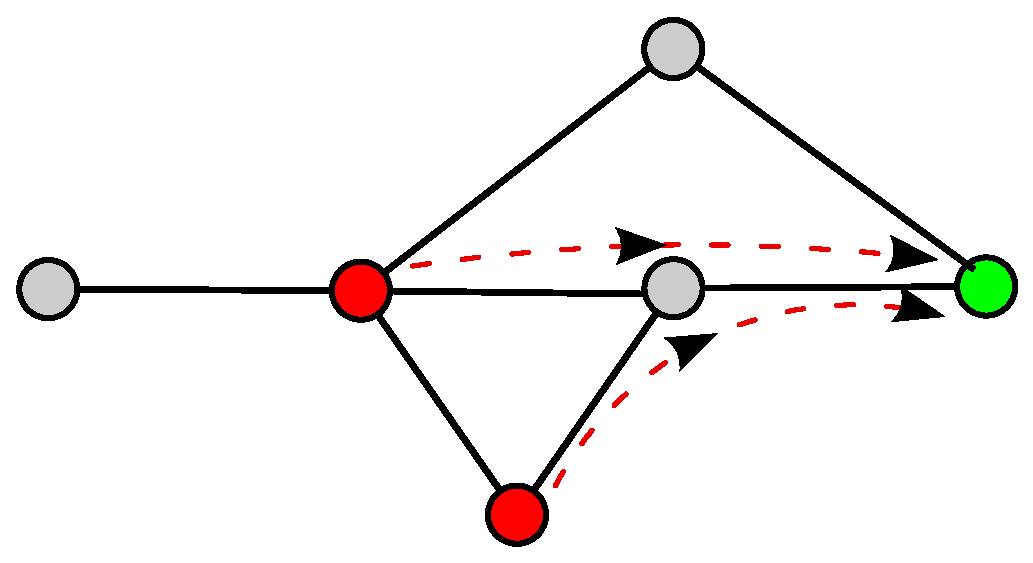
\includegraphics[scale=0.5]{netshort.eps}

\vspace{5 mm}
There is no method specific parameter for NetShort, however note that 
algorithm uses the phenotypic association scores in the edge scores file 
(\textit{edge\_file}) rather than the node scores file (e.g. the average of 
the scores of the nodes the edge in concern connects). A python script to 
create netshort specific edge scores file is provided for convenience (see
below).

\vspace{5 mm}
Thus an example NetShort run would be;

\begin{SaveVerbatim}{bash}
\$> ./guild -s d -n data/test_proteins.txt -e data/test_interactions_for_netshort.txt -o output.txt
\end{SaveVerbatim}
\printcommand{bash}

\vspace{5 mm}
A python script named ``convert\_network\_for\_netshort.py'' is provided 
for creating edge scores file that is going to be used by NetShort 
(where original edge scores are multiplied by average of the scores of the 
nodes the edges belong to). It requires \textit{Python} (version 2.5.2 or 
higher). The following command would convert the original edge scores file 
``data/test\_interactions.txt'' to a NetShort specific 
``data/test\_interactions\_for\_netshort.txt'' egde scores file using node
scores information in ``data/test\_proteins.txt''.

\begin{SaveVerbatim}{bash}
\$> python src/convert_network_for_netshort.py data/test_proteins.txt data/test_interactions.txt 
	data/test_interactions_for_netshort.txt
\end{SaveVerbatim}
\printcommand{bash}


\subsection{fFlow}
In fFlow (based on the algorithm of Functional Flow in Nabieva et al. 2005), 
at each iteration, annotation scores flow from nodes with higher score towards 
nodes with lower scores at the amount of the capacity of the edge through which 
the nodes are connected.

\vspace{5 mm}
The method specific parameters for fFlow are;
\begin{description}
    \item[number\_of\_iterations:] Number of iterations to apply the scoring 
	step of the prioritization algorithm. 
    \item[seed\_score\_threshold:] All the nodes that have higher than this 
	given threshold score will be considered as seeds for the method and 
	assigned infinite scores during scoring.
\end{description}

% Suggested number of iterations is 5.

An example call of fFlow where all nodes that have a score higher than $1.0$ are seeds is;

\begin{SaveVerbatim}{bash}
\$> ./guild -s f -n data/test_proteins.txt -e data/test_interactions.txt -o output.txt -i 5 -t 1.0
\end{SaveVerbatim}
\printcommand{bash}

\subsection{NetRank}
NetRank (based on the ToppGene algorithm proposed by Chen et al. 2009) uses 
Page Rank with priors algorithm (where a random surfer is more likely to end 
up in initially relevant nodes) to score a node in terms of phenotypic 
relevance. The damping factor is 0.15 and the number iterations for convergence 
is defined by the number\_of\_iterations parameter (see below).

\vspace{5 mm}
The method specific parameter for NetRank is;
\begin{description}
    \item[number\_of\_iterations:] Number of iterations to apply the scoring step of the prioritization algorithm. In the case of Page Rank algorithm it defines the number of the times for calculating page ranks for the nodes (convergence criterion for the algorithm). This number is set to 20 by default.
\end{description}

Therefore an example run for NetRank is as follows:

\begin{SaveVerbatim}{bash}
\$> ./guild -s r -n data/test_proteins.txt -e data/test_interactions.txt -o output.txt
\end{SaveVerbatim}
\printcommand{bash}

\subsection{NetWalk}
NetWalk (based on the Random walk with restarts algorithm proposed by Kohler, 
et al., 2008) iteratively simulates random transitions of a walker from a node 
to a randomly selected neighbour node and where at any time step the walk can 
be restarted depending on a predefined probability. Random walk with restarts 
is slightly different than PageRank with priors in the way that it normalizes 
the link weights. The convergence is decided by either having a probability 
difference less than 10e-6 between two consecutive time steps or achieving the 
limit of the number of iterations, set to 50 (though in practice less than 20 
iterations are typically sufficient to satisfy the first criterion). There is 
no method specific parameter for NetWalk.

\vspace{5 mm}
Therefore an example run for NetWalk is as follows:

\begin{SaveVerbatim}{bash}
\$> R --slave --args data/test_proteins.txt data/test_interactions.txt output.txt < random_walk.r
\end{SaveVerbatim}
\printcommand{bash}

\subsection{NetProp}
NetProp (based on the Network propagation algorithm proposed by Vanunu, et al., 
2010) modifies random walk with restarts such that the link weight is 
normalized not only by number of outgoing edges but also by number of incoming 
edges. The convergence is decided as it is done for NetWalk. There is no 
method specific parameter for NetProp.

\vspace{5 mm}
Therefore an example run for NetProp is as follows:

\begin{SaveVerbatim}{bash}
\$> R --slave --args data/test_proteins.txt data/test_interactions.txt output.txt 1 < random_walk.r
\end{SaveVerbatim}
\printcommand{bash}

\subsection{NetCombo}
NetCombo combines the output scores from NetScore, NetZcore and NetShort in 
a consensus scheme by averaging normalized scores (z-scores) of a node in
all of these methods. It requires the output files of NetScore, NetZcore and 
NetShort. 

\vspace{5 mm}
Therefore an example run for NetCombo is as follows:

\begin{SaveVerbatim}{bash}
\$> python src/combine_scores.py output_netscore.txt output_netzcore.txt output_netshort.txt output.txt
\end{SaveVerbatim}
\printcommand{bash}

%\end{multicols}

\end{document}

